\documentclass{beamer}

\usepackage[T1]{fontenc}       
\usepackage[utf8]{inputenc}    % pour les accents (mettre latin1 pour windows au lieu de utf8)
\usepackage[frenchb]{babel}    % le documents est en français
\usepackage{amsmath}           % un packages mathématiques
\usepackage{xcolor}            % pour définir plus de couleurs 
\usepackage{graphicx}          % pour insérer des figures
\usepackage{beamerthemesplit}

\setbeamercovered{transparent}
\usetheme[width=70pt,hideothersubsections]{Hannover}
\setbeamertemplate{footline}[frame number]

\setbeamertemplate{headline}{\hskip 0.2cm \insertlogo }
\setbeamercolor*{titlelike}{parent=structure}

\useinnertheme{circles}
\setbeamertemplate{frametitle}[default][right]
\setbeamertemplate{blocks}[rounded][shadow=true]

%proper colored links
\definecolor{links}{HTML}{2A1B81}
\hypersetup{colorlinks,linkcolor=,urlcolor=links}


%Title info
\title[OAR Cloud]{OAR Cloud - Une infrastructure légère de Cloud Computing basée sur OAR}
\logo{%
  \centering{
    \vspace{0.1cm}%
    
\includegraphics[width=1cm,height=0.5cm,keepaspectratio]{img/logo_pg2009.png}~%
    
\includegraphics[width=0.8cm,height=0.5cm,keepaspectratio]{img/logo_INRIA.png}%
  }
}
\institute{Polytech Grenoble, INRIA\\\scalebox{2}{\insertlogo}}
\author{Michael Mercier}
\date{2013}



% Faire apparaître un sommaire avant chaque section
\AtBeginSection[]{
   \begin{frame}
   \begin{center}{\Large Plan }\end{center}
   %%% affiche en début de chaque section, les noms de sections et
   %%% noms de sous-sections de la section en cours.
   \tableofcontents[currentsection, hideallsubsections]
   \end{frame} 
}
		

% Début de la présentation
% Contenu
\begin{document}
	% Page de titre
	\begin{frame}
		\titlepage
	\end{frame}
	
	
	% Sommaire
	\begin{frame} 
		\begin{center}{\Large Plan }\end{center}
		\tableofcontents[hidesubsections]
	\end{frame}
	
	
  \section{Projet OAR Cloud}
		\begin{frame}
			\frametitle{OAR Cloud}
			\begin{figure}
			  
\includegraphics[scale=0.3]{img/logo_oar.png}
 			\end{figure}
			Les objectifs du projet
			\begin{itemize}
			  \item Définition plus précise du sujet
			  \item Etat de l'art
			  \item Test des technologies émergentes
			  \item Identification des problèmes
			  \item Conception de l'architecture générale
			\end{itemize}			
		\end{frame}
			
			
			
	\section{Le Cloud Computing}
	
		\subsection{Définitions}
			\begin{frame}
			  \frametitle{Cloud computing}
			    \begin{block}{Wikipedia}
			      \textit{Le Cloud computing est l'accès via un réseau de télécommunications, à la demande et en libre-service, à des ressources informatiques partagées configurables}
			    \end{block}
			    Basé sur une pile de services
			    \begin{description}
			      \item[IaaS \textit{Infrastructure as a Service}] 
			      Fournit un accès aux ressources informatiques simple et adaptable aux besoins
			      \item[PaaS \textit{Platform as a Service}]
			      Fournit une plateforme pour faire tourner du code utilisateur
			      \item[SaaS \textit{Software as a Service}]
			      Fournit directement des applications
			    \end{description}
			\end{frame}
			
		\subsection{Gestion des ressources}
			\begin{frame}
				\frametitle{Gestion des ressources}
				\begin{figure}
			    
\includegraphics[scale=0.3]{img/logo_oar.png}
 			  \end{figure}
 			  \textbf{OAR}
 			  \begin{itemize}
   			  \item Gestionnaire de ressources informatiques
   			  \item Dédié au HPC
   			  \item Stable et bien testé
   			  \item Utilisé à grande échelle (Ex: Grid5000)
 			  \end{itemize}
			\end{frame}
	
		\subsection{Virtualisation système}
			\begin{frame}
			  \frametitle{Virtualisation système}
			  \begin{itemize}
   			  \item Décorélation du hardware et du software
			    \item Solutions basées sur différents types d'hyperviseur
			  \end{itemize}
        \begin{figure}
			    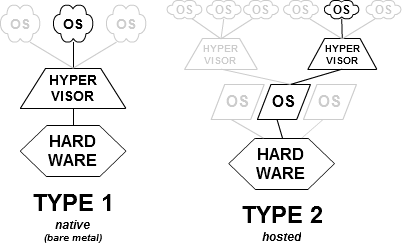
\includegraphics[scale=0.5]{img/Hyperviseur.png}
 			  \end{figure}
 			  \begin{columns}
          \begin{column}{.48\textwidth}
			      \textbf{Type1} Sur le hardware
			    \end{column}
          \hfill
          \begin{column}{.48\textwidth}
            \textbf{Type2} Au dessus de l'OS
          \end{column}
        \end{columns}
			\end{frame}
			
			\begin{frame}
				\frametitle{LXC}
				\textbf{LXC pour LinuX Containers}: Système de virtualisation basé sur l'isolation
				\begin{exampleblock}{Avantages}
				  \begin{itemize}
				    \item Très rapide
				    \item Très configurable
				  \end{itemize}
				\end{exampleblock}
				\begin{alertblock}{Inconvénients}
				  \begin{itemize}
				    \item pas encore sécurisé
				    \item complexe à configurer
				    \item API non stabilisée (version 0.9)
				  \end{itemize}
				\end{alertblock}
			\end{frame}
	
		\subsection{Virtualisation réseaux}
			\begin{frame}
			  \frametitle{Virtualisation réseaux}
			  Basée sur des interfaces logicielles
			  \begin{itemize}
				    \item Isolation des réseaux dans une même machine
				    \item Moins de matériel réseau
				    \item Facilement configurable
				    \item Ex: software-defined networking (SDN)
				\end{itemize}
				\begin{block}{Outils}
				  \begin{itemize}
				      \item Linux Bridge
				      \item OpenVSwitch
				  \end{itemize}
				\end{block}
			\end{frame}
			
			
	\section{Gestion de projet}
	
		\subsection{Déroulement}
			\begin{frame}
			  \frametitle{Déroulement du projet}
			  \begin{itemize}
			    \item Se documenter sur les outils et le contexte
			    \begin{itemize}
			      \item Compréhension et état de l'art du Cloud Computing
			      \item Prise en main d'OAR
			      \item Découverte de LXC
			    \end{itemize}
			    \item Préciser le sujet
			    \item Répartition du travail
			    \begin{itemize}
			      \item Jordan: LXC
            \item Alexandre: OpenVSwitch
            \item Moi: OAR et architecture globale
			    \end{itemize}
			    \item ...
			  \end{itemize}
			\end{frame}
			\begin{frame}
			  \begin{itemize}
			    \item ...
			    \item Conception d'une solution globale
			    \begin{itemize}
			      \item Basée sur le standard: Amazon EC2
            \item Définitions des fonctionnalités
            \item Vue logique
			    \end{itemize}
			    \item Mise en place des jalons
			    \begin{itemize}
			      \item M1: lancer un conteneur LXC dans un job OAR
            \item M2: utiliser OpenVSwitch comme bridge pour 2 conteneurs
            \item M3: coupler les deux précédents jalons
			    \end{itemize}
			    \item Réalisation des jalons
			    \begin{itemize}
			      \item Identification des problèmes
            \item Evaluation des technologies
            \item Ajustement du prochain jalon en fonction
			    \end{itemize}
			  \end{itemize}
			\end{frame}
			
		\subsection{Conception}
			\begin{frame}
				\frametitle{version 0.1}
				\begin{figure}
			    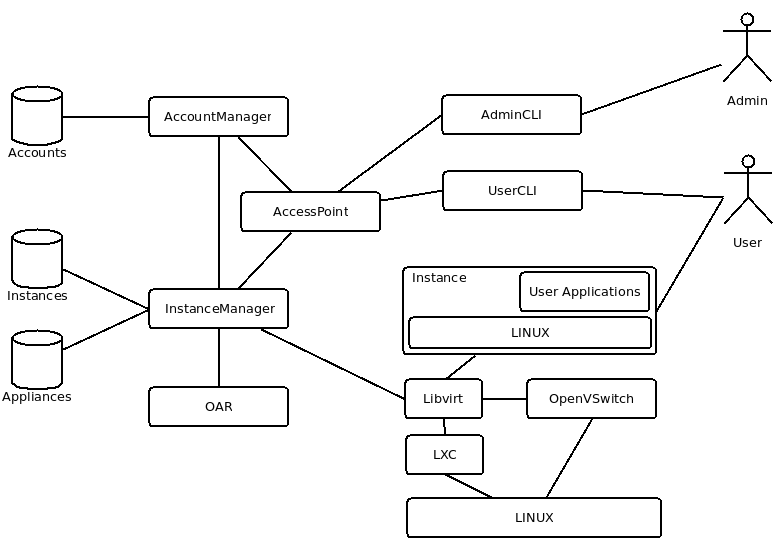
\includegraphics[scale=0.33]{img/DiagLogic_0_1.png}
 			  \end{figure}
			\end{frame}
			\begin{frame}
				\frametitle{version 0.3}
				\begin{figure}
			    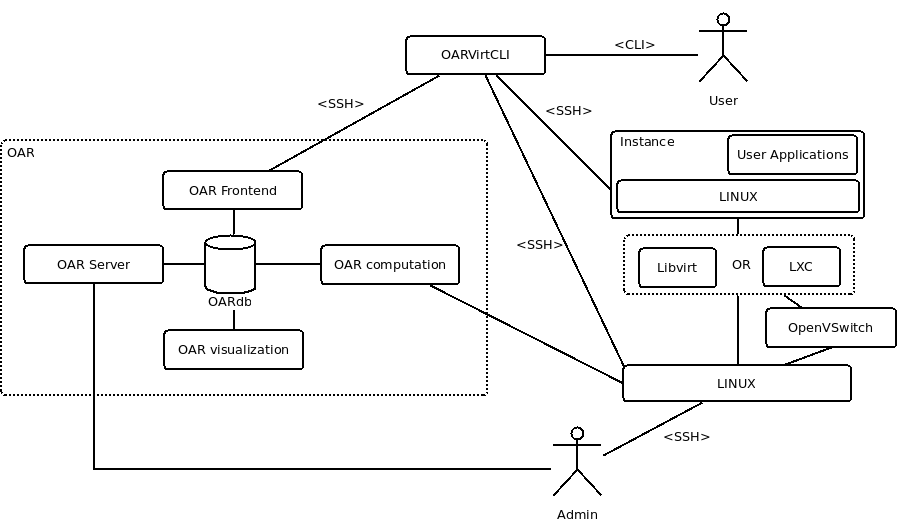
\includegraphics[scale=0.3]{img/DiagLogic_0_3.png}
 			  \end{figure}
			\end{frame}
		
		\subsection{Organisation du travail}
			\begin{frame}
			  \frametitle{Organisation du travail}
			  \begin{itemize}
			    \item Gestion d'équipe
			    \begin{itemize}
			      \item Une réunion par semaine
			      \item Transmission du savoir à travers le \href{http://air.imag.fr/mediawiki/index.php/Proj-2012-2013-OAR-Cloud}{wiki du projet}
			      \item Dépot git sur \href{https://github.com/mickours/oar-cloud}{github}
			    \end{itemize}
			  \end{itemize}
			  \begin{alertblock}{Coopération avec les RICM 4}
			    \begin{itemize}
			      \item Manque de temps à consacrer au projet
			      \item Différences d'investissement au sein de l'équipe
			    \end{itemize}
			    $\Rightarrow$ Très peu de travail en équipe
			  \end{alertblock}
			\end{frame}
		
	\section{Demo}
	
	\section{Bilans}
	  \subsection{Bilan technique}
	    \begin{frame}
        \frametitle{Bilan technique}
		    \begin{itemize}
		      \item M1
		      \begin{itemize}
		        \item LXC est encore en travaux 
		        \item OAR entre en conflit avec LXC sur les cgroups
   		      \item Résolution du conflit possible en modifiant OAR
   		      \item Alternative: KVM (fonctionne avec OpenVSwitch) 
		      \end{itemize}
		      \item M2
		      \begin{itemize}
		        \item En conflit avec les bridges Linux
		        \item OpenVswitch ne fonctionne pas correctement avec LXC
		        \item Problème réglé dans les nouvelles versions?
		        \item Alternative: bridge Linux et OpenFlow
		      \end{itemize}
		    \end{itemize}
	    \end{frame}
	    
	  \subsection{Bilan personnel} 
	    \begin{frame}
        \frametitle{Bilan personnel}
		    \begin{itemize}
		      \item Travail à domicile
		      \item Gestion d'équipe difficile dans ces conditions
		      \item Enormément de connaissances acquises
		      \item Prêt pour le stage!
		    \end{itemize}
	    \end{frame}
		
\end{document}
